\documentclass{article}

\usepackage{graphicx}
\usepackage{tikz}
\usepackage{tikzsymbols}
\usetikzlibrary{calc,patterns,shapes.geometric}
\pagestyle{empty}
\usepackage[margin=0pt]{geometry}
\geometry{papersize={14in,12in}}

\def\centerarc[#1](#2)(#3:#4:#5){\draw[#1] ($(#2)+({#5*cos(#3)},{#5*sin(#3)})$) arc (#3:#4:#5);}

\begin{document}
	\begin{figure}
		\centering
		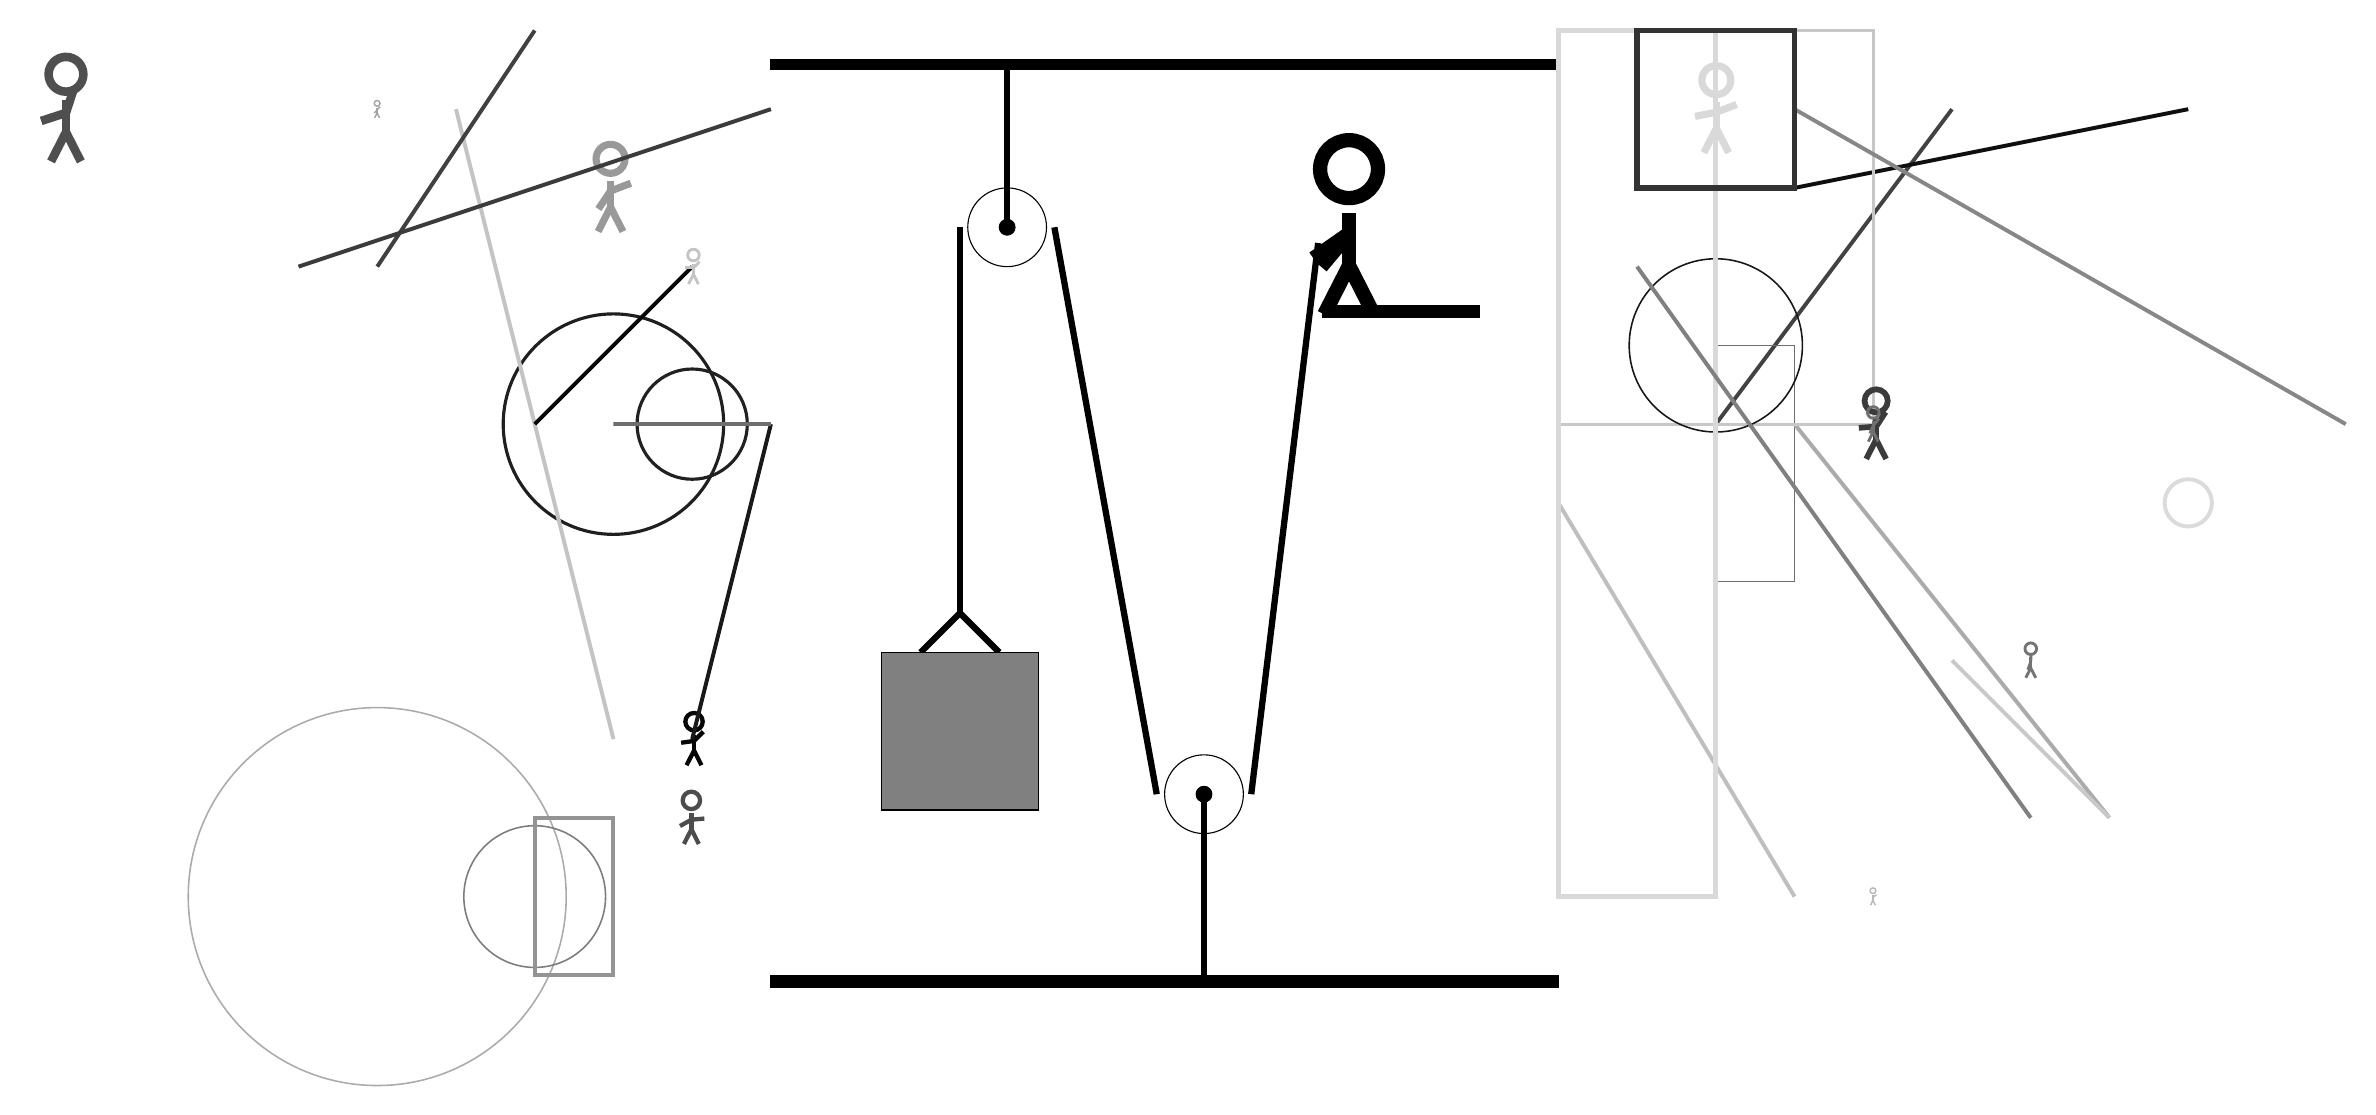
\begin{tikzpicture}
			%%%%% START %%%%%
			
			\draw[fill=black] (-2, 11.5) rectangle (8, 11.625);
			
			\draw (3.5, 2.3) circle (0.5);
			\draw[fill=black] (3.5, 2.3) circle (0.1);
			\draw[line width=0.8mm] (3.5, 2.3) -- (3.5, 0);
			
			\draw [line width=0.4mm, color=black!88](-4, 7) circle (1.4);
			
			\draw[line width=0.5mm, color=black!74](13, 11) -- (10, 7);
			\node[line width=0.7mm, color=black!70] at (-3, 2) {\Strichmaxerl[3][29][5]};
			\draw[line width=0.2mm, color=black!57] (10, 8) rectangle (11, 5);
			\node[line width=0.5mm, color=black!15] at (10, 11) {\Strichmaxerl[5][11][21]};
			\node[line width=0.5mm, color=black!98] at (-3, 3) {\Strichmaxerl[3][8][45]};
			
			\draw[line width=0.5mm, color=black!23](-4, 3) -- (-6, 11);
			
			\node[line width=0.4mm, color=black!36] at (-7, 11) {\Strichmaxerl[1][48][45]};
			\draw[line width=0.5mm, color=black!75](-7, 9) -- (-5, 12);
			
			\draw[line width=0.5mm, color=black!97](-5, 7) -- (-3, 9);
			\draw[line width=0.5mm, color=black!94](11, 10) -- (16, 11);
			\draw[line width=0.5mm, color=black!33](11, 7) -- (15, 2);
			\draw[line width=0.5mm, color=black!25](11, 1) -- (8, 6);
			\draw[line width=0.4mm, color=black!22] (8, 7) rectangle (12, 12);
			\draw [line width=0.2mm, color=black!91](10, 8) circle (1.1);
			\draw[line width=0.5mm, color=black!47](11, 11) -- (18, 7);
			
			\node[line width=0.5mm, color=black!77] at (12, 7) {\Strichmaxerl[4][4][57]};
			
			\node[line width=0.2mm, color=black!40] at (-4, 10) {\Strichmaxerl[5][56][21]};
			\draw[line width=0.6mm, color=black!15] (8, 12) rectangle (10, 1);
			
			\draw[line width=0.5mm, color=black!90](-2, 7) -- (-3, 3);
			\draw [line width=0.2mm, color=black!33](-7, 1) circle (2.4);
			
			\draw [line width=0.5mm, color=black!14](16, 6) circle (0.3);
			\draw [line width=0.4mm, color=black!87](-3, 7) circle (0.7);
			\node[line width=0.6mm, color=black!69] at (-11, 11) {\Strichmaxerl[6][18][72]};
			\draw[line width=0.5mm, color=black!50](9, 9) -- (14, 2);
			
			\draw[line width=0.6mm, color=black!57] (-4, 7) rectangle (-2, 7);
			\node[line width=0.4mm, color=black!28] at (12, 1) {\Strichmaxerl[1][84][34]};
			\draw [line width=0.2mm, color=black!51](-5, 1) circle (0.9);
			\node[line width=0.6mm, color=black!56] at (12, 7) {\Strichmaxerl[2][67][50]};
			\node[line width=0.7mm, color=black!23] at (-3, 9) {\Strichmaxerl[2][0][45]};
			\draw[line width=0.5mm, color=black!42] (-4, 2) rectangle (-5, 0);
			
			\draw[line width=0.5mm, color=black!21](13, 4) -- (15, 2);
			\draw[line width=0.7mm, color=black!80] (9, 10) rectangle (11, 12);
			\draw[line width=0.5mm, color=black!77](-2, 11) -- (-8, 9);
			\node[line width=0.4mm, color=black!55] at (14, 4) {\Strichmaxerl[2][71][88]};
			
			\draw (1, 9.5) circle (0.5);
			\draw[fill=black] (1, 9.5) circle (0.1);
			\draw[line width=0.8mm] (1, 11.5) -- (1, 9.5);
			
			\draw[line width=0.8mm](-0.1, 4.1) --  (0.4, 4.6) -- (0.9, 4.1);
			\draw[fill=black!50] (-0.6, 4.1) rectangle (1.4, 2.1);
			
			\draw[line width=0.8mm](0.4, 9.5) -- (0.4, 4.6);
			\centerarc[line width=0.8mm](1, 9.5)(180:0:0.6)
			\draw[line width=0.8mm](1.6, 9.5) -- (2.9, 2.3);
			\centerarc[line width=0.8mm](3.5, 2.3)(180:360:0.6)
			\draw[line width=0.8mm](4.1, 2.3) -- (4.95, 9.3);
			
			\node at (5.3, 9.5) {\Strichmaxerl[10][35][-130]};
			\draw[fill=black] (5, 8.5) rectangle (7, 8.35);
			
			\draw[fill=black] (-2, 0) rectangle (8, -0.15);
			
			%%%%% END %%%%%
		\end{tikzpicture}
	\end{figure}	
\end{document}